\documentclass{article}%
\usepackage[T1]{fontenc}%
\usepackage[utf8]{inputenc}%
\usepackage{lmodern}%
\usepackage{textcomp}%
\usepackage{lastpage}%
\usepackage{parskip}%
\usepackage[top=1.2in,bottom=1in,left=0.6in,right=0.6in,headsep=0.8in]{geometry}%
\usepackage{amsmath}%
\usepackage{graphicx}%
\usepackage{needspace}%
\usepackage{color}%
\usepackage{longtable}%
\usepackage{multirow}%
\usepackage[table]{xcolor}%
\usepackage{fancyhdr}%
\usepackage{tabularx}%
%
\definecolor{OsdagGreen}{HTML}{D5DF93}%
\fancypagestyle{header}{ 
\renewcommand{\headrulewidth}{0pt}%
\renewcommand{\footrulewidth}{0pt}%
\fancyhead{ 
}%
\fancyfoot{ 
}%
\fancyhead[C]{ 
\begin{tabularx}{\textwidth}{|l|p{6cm}|l|X|}%
\hline%
\rowcolor{OsdagGreen}%
Company Name&LoremIpsum&Project Title&Fossee\\%
\hline%
\rowcolor{OsdagGreen}%
Group/Team Name&LoremIpsum&Subtitle&\\%
\hline%
\rowcolor{OsdagGreen}%
Designer&LoremIpsum&Job Number&123\\%
\hline%
\rowcolor{OsdagGreen}%
Date&29 /04 /2020&Client&LoremIpsum\\%
\hline%
\end{tabularx}
}%
\fancyfoot[R]{ 
Page \thepage\ of \pageref{LastPage}
}
}%
%
\begin{document}%
\normalsize%
\pagestyle{header}%
\section{Input Parameters}%
\label{sec:InputParameters}%
\renewcommand{\arraystretch}{1.2}%
\begin{longtable}{|p{5cm}|p{2cm}|p{2cm}|p{2cm}|p{5cm}|}%
\hline%
\hline%
\multicolumn{3}{|c|}{Module}&\multicolumn{2}{|c|}{Fin Plate}\\%
\hline%
\hline%
\multicolumn{3}{|c|}{MainModule}&\multicolumn{2}{|c|}{Shear Connection}\\%
\hline%
\hline%
\multicolumn{3}{|c|}{Connectivity}&\multicolumn{2}{|c|}{Column flange{-}Beam web}\\%
\hline%
\hline%
\multicolumn{3}{|c|}{Shear(kN)*}&\multicolumn{2}{|c|}{30.0}\\%
\hline%
\hline%
\multicolumn{5}{|c|}{\textbf{Supporting Section}}\\%
\hline%
\hline%
\multirow{13}{*}{\includegraphics[width=5cm,height=5cm]{"C:/Users/nitin/Pictures/Saved Pictures/Osdag3/ResourceFiles/images/ISection".png}}&\multicolumn{2}{|c|}{Supporting Section}&\multicolumn{2}{|c|}{PBP 300X222.9}\\%
\cline{2%
-%
5}%
&\multicolumn{2}{|c|}{Material *}&\multicolumn{2}{|c|}{E 250 (Fe 410 W)A}\\%
\cline{2%
-%
5}%
&\multicolumn{2}{|c|}{Ultimate strength, fu (MPa)}&\multicolumn{2}{|c|}{410}\\%
\cline{2%
-%
5}%
&\multicolumn{2}{|c|}{Yield Strength , fy (MPa)}&\multicolumn{2}{|c|}{230}\\%
\cline{2%
-%
5}%
&Mass&222.92&Iz(cm4)&526988000.0\\%
\cline{2%
-%
5}%
&Area(cm2) {-} A&28400.0&Iy(cm4)&175746300.0\\%
\cline{2%
-%
5}%
&D(mm)&337.9&rz(cm)&136.2\\%
\cline{2%
-%
5}%
&B(mm)&325.7&ry(cm)&78.7\\%
\cline{2%
-%
5}%
&t(mm)&30.3&Zz(cm3)&3119190.0\\%
\cline{2%
-%
5}%
&T(mm)&30.4&Zy(cm3)&1079190.0\\%
\cline{2%
-%
5}%
&FlangeSlope&90&Zpz(cm3)&3653090.0\\%
\cline{2%
-%
5}%
&R1(mm)&1.52&Zpy(cm3)&1079190.0\\%
\cline{2%
-%
5}%
&R2(mm)&0.0&&\\%
\cline{2%
-%
5}%
\hline%
\multicolumn{5}{|c|}{\textbf{Supported Section}}\\%
\hline%
\hline%
\multirow{13}{*}{\includegraphics[width=5cm,height=5cm]{"C:/Users/nitin/Pictures/Saved Pictures/Osdag3/ResourceFiles/images/ISection".png}}&\multicolumn{2}{|c|}{Supported Section}&\multicolumn{2}{|c|}{LB 300}\\%
\cline{2%
-%
5}%
&\multicolumn{2}{|c|}{Material *}&\multicolumn{2}{|c|}{E 250 (Fe 410 W)A}\\%
\cline{2%
-%
5}%
&\multicolumn{2}{|c|}{Ultimate strength, fu (MPa)}&\multicolumn{2}{|c|}{410}\\%
\cline{2%
-%
5}%
&\multicolumn{2}{|c|}{Yield Strength , fy (MPa)}&\multicolumn{2}{|c|}{230}\\%
\cline{2%
-%
5}%
&Mass&37.7&Iz(cm4)&73300000.0\\%
\cline{2%
-%
5}%
&Area(cm2) {-} A&4810.0&Iy(cm4)&3760000.0\\%
\cline{2%
-%
5}%
&D(mm)&300.0&rz(cm)&124.0\\%
\cline{2%
-%
5}%
&B(mm)&150.0&ry(cm)&28.0\\%
\cline{2%
-%
5}%
&t(mm)&6.7&Zz(cm3)&489000.0\\%
\cline{2%
-%
5}%
&T(mm)&9.4&Zy(cm3)&50200.0\\%
\cline{2%
-%
5}%
&FlangeSlope&98&Zpz(cm3)&489000.0\\%
\cline{2%
-%
5}%
&R1(mm)&15.0&Zpy(cm3)&50200.0\\%
\cline{2%
-%
5}%
&R2(mm)&7.5&&\\%
\cline{2%
-%
5}%
\hline%
\multicolumn{5}{|c|}{\textbf{Bolt Details}}\\%
\hline%
\hline%
\multicolumn{3}{|c|}{Diameter(mm)*}&\multicolumn{2}{|c|}{{[}12.0, 16.0, 20.0, 24.0, 30.0, 36.0{]}}\\%
\hline%
\hline%
\multicolumn{3}{|c|}{Grade *}&\multicolumn{2}{|c|}{{[}3.6, 4.6, 4.8, 5.6, 5.8, 6.8, 8.8, 9.8, 10.9, 12.9{]}}\\%
\hline%
\hline%
\multicolumn{3}{|c|}{Type *}&\multicolumn{2}{|c|}{Bearing Bolt}\\%
\hline%
\hline%
\multicolumn{3}{|c|}{Bolt hole type}&\multicolumn{2}{|c|}{Standard}\\%
\hline%
\hline%
\multicolumn{3}{|c|}{Slip factor (µ\_f)}&\multicolumn{2}{|c|}{0.3}\\%
\hline%
\hline%
\multicolumn{3}{|c|}{Type of edges}&\multicolumn{2}{|c|}{a {-} Sheared or hand flame cut}\\%
\hline%
\hline%
\multicolumn{3}{|c|}{Gap between beam and <br>support (mm)}&\multicolumn{2}{|c|}{10.0}\\%
\hline%
\hline%
\multicolumn{3}{|c|}{Are the members exposed to <br>corrosive influences}&\multicolumn{2}{|c|}{False}\\%
\hline%
\hline%
\multicolumn{5}{|c|}{\textbf{Weld Details}}\\%
\hline%
\hline%
\multicolumn{3}{|c|}{Weld Type}&\multicolumn{2}{|c|}{Fillet}\\%
\hline%
\hline%
\multicolumn{3}{|c|}{Type of weld fabrication}&\multicolumn{2}{|c|}{Shop Weld}\\%
\hline%
\hline%
\multicolumn{3}{|c|}{Material grade overwrite (MPa) Fu}&\multicolumn{2}{|c|}{410.0}\\%
\hline%
\end{longtable}

%
\Needspace{10\baselineskip}%
\section{Design Checks}%
\label{sec:DesignChecks}%
\subsection{Bolt Design Checks}%
\label{subsec:BoltDesignChecks}%
\renewcommand{\arraystretch}{1.2}%
\begin{longtable}{|p{4cm}|p{5cm}|p{5.5cm}|p{1.5cm}|}%
\hline%
\rowcolor{OsdagGreen}%
Check&Required&Provided&Remarks\\%
\hline%
\endhead%
\hline%
Shear Capacity (kN)&&$\begin{aligned}V_{dsb} &= \frac{f_ub ~n_n~ A_{nb}}{\sqrt{3} ~\gamma_{mb}}\\ &= \frac{410*1*84.3}{\sqrt{3}~*~1.25}\\ &= 31.15\end{aligned}$&\\%
\hline%
Bearing Capacity (kN)&&$\begin{aligned}V_{dpb} &= \frac{2.5~ k_b~ d~ t~ f_u}{\gamma_{mb}}\\ &= \frac{2.5~*0.52*12.0*6.7*410}{1.25}\\ &=31.15\end{aligned}$&\\%
\hline%
Capacity (KN)&&$\begin{aligned}V_{db} &= min~ (V_{dsb}, V_{dpb})\\ &= min~ (31.15,31.15)\\ &=31.15\end{aligned}$&\\%
\hline%
No of Bolts&$\begin{aligned}R_{u} &= \sqrt{V_u^2+A_u^2}\\ n_{trial} &= R_u/ V_{bolt}\\ R_{u} &= \frac{\sqrt{30.0^2+30.0^2}}{31.15}\\ &=2\end{aligned}$&2&\\%
\hline%
No of Columns&&1&\\%
\hline%
No of Rows&&2&\\%
\hline%
Min. Pitch (mm)&$\begin{aligned}p/g_{min}&= 2.5 ~ d&\\ =&2.5*12.0&=30.0\end{aligned}$&0.0&N/A\\%
\hline%
Max. Pitch (mm)&$\begin{aligned}p/g_{max} &=\min(32~t,~300~mm)&\\ &=\min(32 *~6.7,~ 300 ~mm)\\&=300\end{aligned}$&0.0&N/A\\%
\hline%
Min. Gauge (mm)&$\begin{aligned}p/g_{min}&= 2.5 ~ d&\\ =&2.5*12.0&=30.0\end{aligned}$&130&Pass\\%
\hline%
Max. Gauge (mm)&$\begin{aligned}p/g_{max} &=\min(32~t,~300~mm)&\\ &=\min(32 *~6.7,~ 300 ~mm)\\&=300\end{aligned}$&130&Pass\\%
\hline%
Min. End Distance (mm)&$\begin{aligned}e/e`_{min} &=[1.5~or~ 1.7] * d_0\\ &=1.7*13.0=22.1 \end{aligned}$&25&Pass\\%
\hline%
Max. End Distance (mm)&$\begin{aligned}e/e`_{max} &= 12~ t~ \varepsilon&\\ \varepsilon &= \sqrt{\frac{250}{f_y}}\\ e/e`_{max}&=12 ~*8.0*\sqrt{\frac{250}{230}}\\ &=99.84\\ \end{aligned}$&25&Pass\\%
\hline%
Min. Edge Distance (mm)&$\begin{aligned}e/e`_{min} &=[1.5~or~ 1.7] * d_0\\ &=1.7*13.0=22.1 \end{aligned}$&25&Pass\\%
\hline%
Max. Edge Distance (mm)&$\begin{aligned}e/e`_{max} &= 12~ t~ \varepsilon&\\ \varepsilon &= \sqrt{\frac{250}{f_y}}\\ e/e`_{max}&=12 ~*8.0*\sqrt{\frac{250}{230}}\\ &=99.84\\ \end{aligned}$&25&Pass\\%
\hline%
Capacity (KN)&27523.52&31149.2&Pass\\%
\hline%
\end{longtable}

%
\subsection{Plate Design Checks}%
\label{subsec:PlateDesignChecks}%
\renewcommand{\arraystretch}{1.2}%
\begin{longtable}{|p{4cm}|p{5cm}|p{5.5cm}|p{1.5cm}|}%
\hline%
\rowcolor{OsdagGreen}%
Check&Required&Provided&Remarks\\%
\hline%
\endhead%
\hline%
Min. Plate Height (mm)&$\begin{aligned}0.6 * d_b&= 0.6 * 300.0=180.0\end{aligned}$&180&Pass\\%
\hline%
Max. Plate Height (mm)&$\begin{aligned} &d_b - 2 (t_{bf} + r_{b1} + gap)\\ &=300.0- 2* (9.4+15.0+ 10)\\ &=251.2\end{aligned}$&180&Pass\\%
\hline%
Min. Plate Length (mm)&$\begin{aligned} &2*e_{min} + (n~c-1) * p_{min})\\ &=2*22.1+(1-1) * 30.0\\ &=54.2\end{aligned}$&60.0&Pass\\%
\hline%
Min.Plate Thickness (mm)&$\begin{aligned} t_w=6.7\end{aligned}$&8.0&Pass\\%
\hline%
Shear yielding Capacity (V\_dy) (kN)&&$\begin{aligned} V_{dg} &= \frac{A_v*f_y}{\sqrt{3}*\gamma_{mo}}\\ &=\frac{180*8.0*230}{\sqrt{3}*1.1}\\ &=104.3\end{aligned}$&\\%
\hline%
Shear Rupture Capacity (V\_dn) (kN)&&$\begin{aligned} V_{dn} &= \frac{0.75*A_{vn}*f_u}{\sqrt{3}*\gamma_{mo}}\\ &=1*(180-(2*13.0))*8.0*410\\ &=378.84\end{aligned}$&\\%
\hline%
Block Shear Capacity in Shear (V\_db) (kN)&&203.04&\\%
\hline%
Shear Capacity (V\_d) (kN)&30.0&$\begin{aligned} V_d &= Min(V_{dy},V_{dn},V_{db})\\ &= Min(104.3,378.84,203.04)\\ &=104.3\end{aligned}$&Pass\\%
\hline%
Tension Yielding Capacity (kN)&&$\begin{aligned} T_{dg} &= \frac{l*t*f_y}{\gamma_{mo}}\\ &=\frac{60.0*8.0*230}{\sqrt{3}*1.1}\\ &=100.36\end{aligned}$&\\%
\hline%
Tension Rupture Capacity(kN)&&$\begin{aligned} T_{dn} &= \frac{0.9*A_{n}*f_u}{\gamma_{m1}}\\ &=\frac{0.9*(60.0-2*13.0)*8.0*410}{1.25}\\ &=111.0\end{aligned}$&\\%
\hline%
Block Shear Capacity in Tension (T\_db) (kN)&&203.04&\\%
\hline%
Tension Capacity (kN)&30.0&$\begin{aligned} T_d &= Min(T_{dg},T_{dn},T_{db})\\ &= Min(100.36,111.0,203.04)\\ &=100.36\end{aligned}$&Pass\\%
\hline%
Moment Capacity (kNm)&1.05&10.84&Pass\\%
\hline%
Interaction Ratio&$\begin{aligned} \leq1\end{aligned}$&$\begin{aligned} \frac{1.05}{10.84}+\frac{30.0}{100.36}=0.4\end{aligned}$&Pass\\%
\hline%
\end{longtable}

%
\subsection{Weld Checks}%
\label{subsec:WeldChecks}%
\renewcommand{\arraystretch}{1.2}%
\begin{longtable}{|p{4cm}|p{7.0cm}|p{3.5cm}|p{1.5cm}|}%
\hline%
\rowcolor{OsdagGreen}%
Check&Required&Provided&Remarks\\%
\hline%
\endhead%
\hline%
Min Weld Size (mm)&$\begin{aligned} Thickness~of~Thicker~part&\\ =Max(30.4,30.4)&=30.4\\ IS800:2007~cl.10.5.2.3~Table 21,&\\ t_{w_{min}} &=6\end{aligned}$&6&Pass\\%
\hline%
Max Weld Size (mm)&$\begin{aligned} Thickness~of~Thinner~part&\\ =Min(30.4,30.4)&=8.0\\ t_{w_{max}} &=8.0\end{aligned}$&6&Pass\\%
\hline%
Weld Strength (kN/mm)&$\begin{aligned} R_w&=\sqrt{(T_{wh}+A_{wh})^2 + (T_{wv}+V_{wv})^2}\\ T_{wh}&=\frac{M*y_{max}}{I{pw}}=\frac{1050000.0*84.0}{790272.0}\\ T_{wv}&=\frac{M*x_{max}}{I{pw}}=\frac{1050000.0*0.0}{790272.0}\\ V_{wv}&=\frac{V}{l_w}=\frac{30000.0}{336}\\ A_{wh}&=\frac{A}{l_w}=\frac{30000.0}{336}\\ R_w&=\sqrt{(111.61+89.29)^2 + (0.0+89.29)^2}\\ &=219.84\end{aligned}$&$\begin{aligned} f_w &=\frac{t_t*f_u}{\sqrt{3}*\gamma_{mw}}\\ &=\frac{4.2*410}{\sqrt{3}}*1.25\\ &=795.36\end{aligned}$&Pass\\%
\hline%
\end{longtable}

%
\Needspace{10\baselineskip}%
\newpage%
\section{3D View}%
\label{sec:3DView}%


\begin{figure}[h!]%
\centering%
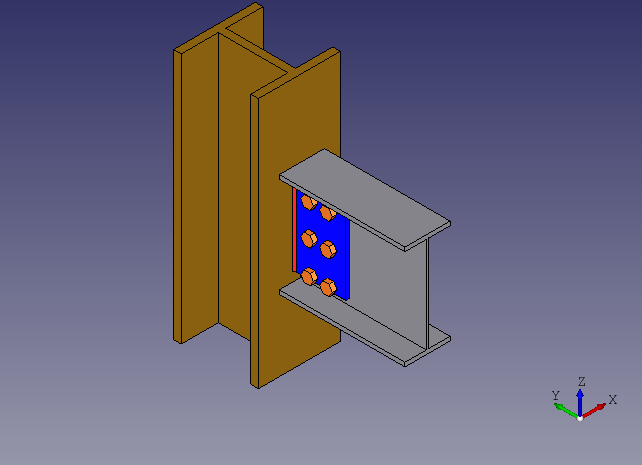
\includegraphics[width=\linewidth]{{"C:/Users/nitin/Pictures/Saved Pictures/Osdag3./ResourceFiles/images/3d}.png}%
\caption{3D View}%
\end{figure}

%
\end{document}